\documentclass[a4paper,12pt]{article}
\usepackage{amsmath, amssymb}
\usepackage{siunitx}
\usepackage{hyperref}
\usepackage{graphicx}
\usepackage{float}
\usepackage[a4paper, top=0.5in, bottom=0.5in, left=1in, right=1in]{geometry}
\usepackage{xcolor}
\usepackage{colortbl}
\usepackage{titlesec}
\usepackage{fontspec}
\usepackage{tikz}
\usepackage{lipsum} % For dummy text, remove this for your actual report
\usepackage{listings}
\usepackage{subcaption}
\usepackage[most]{tcolorbox}
\usepackage{fancyhdr}
\lstset{
    language=Python,        % Specify the language
    basicstyle=\ttfamily,   % Basic font style
    keywordstyle=\color{blue}\bfseries, % Keywords style
    commentstyle=\color{green},         % Comments style
    stringstyle=\color{red},            % Strings style
    numbers=left,                      % Add line numbers
    numberstyle=\tiny,                 % Line number style
    stepnumber=1,                      % Step between line numbers
    frame=single,                      % Add a frame around the code
    breaklines=true                    % Allow breaking long lines
}

\definecolor{myblue}{rgb}{0.1, 0.2, 0.7}
\definecolor{mygreen}{rgb}{0.1, 0.6, 0.1}
\definecolor{myred}{rgb}{0.7, 0.2, 0.2}
\definecolor{lightblue}{rgb}{0.8, 0.9, 1}
\definecolor{mygold}{rgb}{0.8, 0.6, 0.1}
\definecolor{mygray}{rgb}{0.9, 0.9, 0.9}

% Customize title formatting
\titleformat{\title}[block]
  {\normalfont\Huge\bfseries\color{myblue}}{}{0em}{}

\titleformat{\author}[block]
  {\normalfont\LARGE\itshape\color{mygreen}}{}{0em}{}

% Custom header line
\newcommand{\myheader}{
    \noindent\rule{\textwidth}{1pt}\\[0.4cm]
}

% Title page design
\begin{document}

% Title Page
\begin{titlepage}
    \centering
    
    \vspace*{2cm}
    
    % Title
    {\Huge \bfseries \textcolor{myblue}{Lab Report : Transient Response of LC circuits}}\\[0.5cm]
    {\LARGE \textit{\textcolor{red}{Analysing the LC circuit response}}\\[1.5cm]
    
    % Author names
    \noindent
    \textbf{\Huge Krishna Patil-EE24BTECH11036}\\[0.3cm]
    \textbf{\Huge Deepak Ahirwar-EE24BTECH11014}\\[1.5cm]
    
    % Institution name
    {\LARGE \textit{Electrical Department, IIT-Hyderabad}}\\[2cm]
    
    \vfill
    
    % Date
    {\LARGE \today}
    
    % Footer - with gradient line and custom footer text
    \vfill
    \myheader
    \centering
    \textcolor{mygold}{\Large \textit{Experiment conducted as part of ELectric Circuits Lab Coursework.}}
    
\end{titlepage}

\pagestyle{fancy}
\fancyhf{}
\rhead{\textcolor{purple}{LC Circuit Analysis}}
\lhead{\textcolor{orange}{Electric Circuits Lab}}
\cfoot{\textcolor{red}{\thepage}}

\begin{tcolorbox}[colframe=red!70!black,colback=yellow!10!white,title=\textbf{\textcolor{red}{Objective}}]
The objective of this experiment is to investigate the transient response of an LC circuit, analyze its oscillatory behavior, determine the natural frequency ($\Omega_n$), and evaluate the damping ratio ($\xi$) using both theoretical and experimental methods.
\end{tcolorbox}

\begin{tcolorbox}[colframe=blue!70!black,colback=cyan!10!white,title=\textbf{\textcolor{blue}{Equipment Required}}]
\begin{itemize}
\item \textcolor{green}{100 $\mu$F capacitor}\item \textcolor{green}{Largest available inductor (denoted as L)}\item \textcolor{green}{Small resistor (for optional damping analysis)}\item \textcolor{green}{DC power supply}\item \textcolor{green}{Digital oscilloscope}\item \textcolor{green}{Function generator}\item \textcolor{green}{Connecting wires and probes}\item \textcolor{green}{Multimeter for component verification}\end{itemize}
\end{tcolorbox}

\section{\textcolor{red}{Theory}}
\subsection{\textcolor{blue}{Mathematical Analysis}}
\begin{tcolorbox}[breakable , colframe=purple!70!black,colback=magenta!10!white]
An LC circuit follows a second-order differential equation:
\begin{equation}
\frac{d^2V}{dt^2} + \frac{R}{L} \frac{dV}{dt} + \frac{1}{LC} V = 0
\end{equation}

For an \textbf{ideal LC circuit} (with zero resistance), the equation reduces to:
\begin{equation}
\frac{d^2V}{dt^2} + \frac{1}{LC} V = 0
\end{equation}
The general solution is given by:
\begin{equation}
V(t) = V_0 \cos(\Omega_n t + \phi)
\end{equation}
where:
\begin{itemize}
\item $\Omega_n = \frac{1}{\sqrt{LC}}$ is the natural frequency,
\item $V_0$ is the initial voltage, and
\item $\phi$ is the phase angle.
\end{itemize}

However, in the \textbf{real world}, resistance ($R$) cannot be ignored. This results in a damped response:
\begin{equation}
\frac{d^2V}{dt^2} + \frac{R}{L} \frac{dV}{dt} + \frac{1}{LC} V = 0
\end{equation}
The solution depends on the damping ratio $\xi = \frac{R}{2} \sqrt{\frac{C}{L}}$:
\begin{itemize}
\item \textbf{Underdamped ($\xi < 1$):}
\begin{equation}
V(t) = V_0 e^{-\xi \Omega_n t} \cos(\Omega_d t + \phi), \quad \Omega_d = \Omega_n \sqrt{1 - \xi^2}
\end{equation}
\item \textbf{Critically damped ($\xi = 1$):}
\begin{equation}
V(t) = (A + Bt) e^{-\Omega_n t}
\end{equation}
\item \textbf{Overdamped ($\xi > 1$):}
\begin{equation}
V(t) = A e^{-s_1 t} + B e^{-s_2 t}, \quad s_{1,2} = \Omega_n (\xi \pm \sqrt{\xi^2 - 1})
\end{equation}
\end{itemize}
\end{tcolorbox}

\section{\textcolor{red}{Real-World Considerations}}
\begin{tcolorbox}[colframe=black!70!black,colback=gray!10!white]
In practical circuits, parasitic resistances from wires, connectors, and components introduce damping. This results in energy loss and prevents perpetual oscillation. The presence of resistance reduces the amplitude over time, transforming the ideal sinusoidal response into a decaying waveform. The real-world transient response is always governed by the damped equation:
\begin{equation}
\frac{d^2V}{dt^2} + \frac{R}{L} \frac{dV}{dt} + \frac{1}{LC} V = 0
\end{equation}
\textcolor{black}{Understanding and accounting for these effects is essential for accurate circuit design and analysis.}
\end{tcolorbox}

\section{\textcolor{red}{Images of Responses}}
\begin{tcolorbox}[breakable , colframe=black!70!black,colback=gray!10!white,title=\textbf{\textcolor{black}{Oscilloscope Waveforms and Circuit Images}}]
\begin{center}
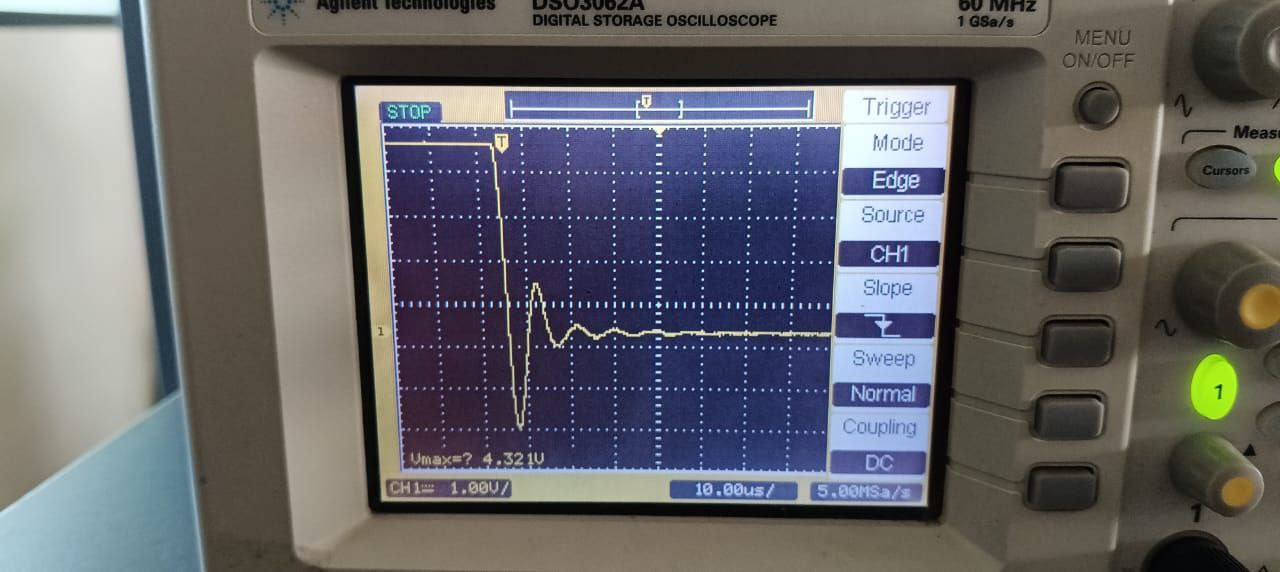
\includegraphics[width=1.0\textwidth]{fig/response_image1.jpg} \
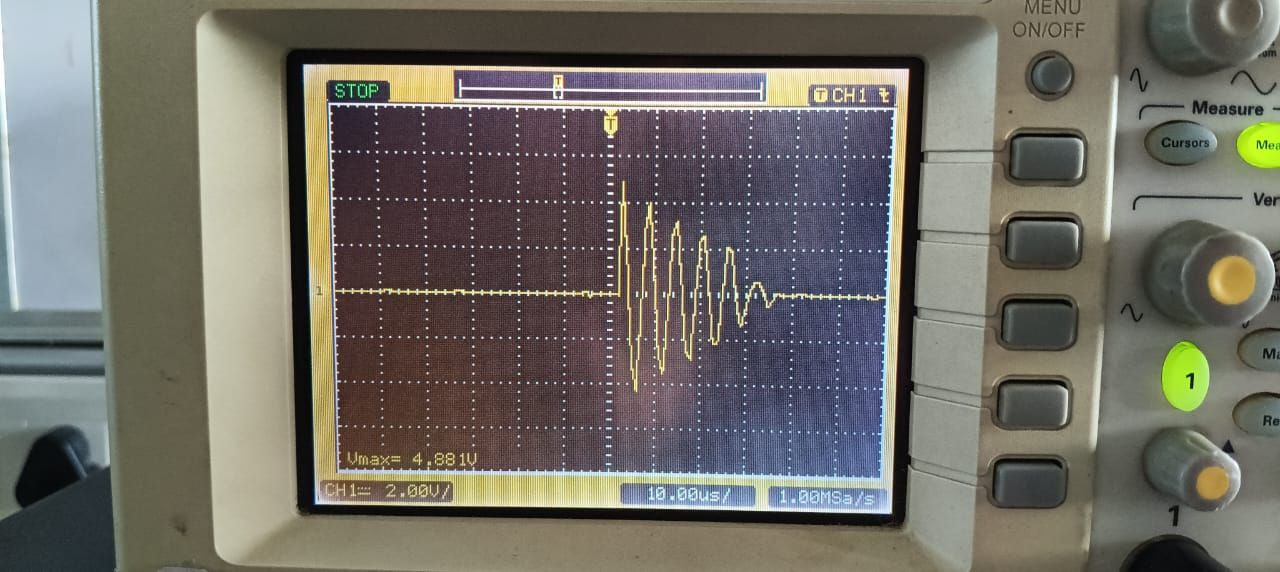
\includegraphics[width=0.8\textwidth]{fig/response_image2.jpg}
\end{center}
\textcolor{black}{Above images depict the transient response captured during the experiment, highlighting differences between ideal and real-world oscillations.}
\end{tcolorbox}

\section{\textcolor{red}{Conclusion}}
\begin{tcolorbox}[colframe=red!70!black,colback=yellow!10!white]
The experimentally observed natural frequency closely matched theoretical values. However, real-world resistance caused measurable damping effects, reducing amplitude over time. This experiment validated that while ideal equations predict behavior accurately, practical factors must be accounted for in realistic scenarios.
\end{tcolorbox}

\section{\textcolor{red}{Safety Precautions}}
\begin{tcolorbox}[colframe=purple!70!black,colback=magenta!10!white]
\begin{itemize}
\item Handle charged capacitors carefully to avoid accidental discharges.
\item Ground the oscilloscope properly for accurate and safe measurements.
\end{itemize}
\end{tcolorbox}

\section{\textcolor{red}{References}}
\begin{tcolorbox}[colframe=green!70!black,colback=yellow!10!white]
\begin{itemize}
\item \textit{Transient Response of an LC Circuit}.
\item Circuit analysis textbooks and academic literature.
\end{itemize}
\end{tcolorbox}

\end{document}


